\documentclass{beamer}

%%%%%%%%%%%%%%%%%%%%%
%%% config
%%%%%%%%%%%%%%%%%%%%%

% ********************************************************************    
% Packages
% ********************************************************************
\usepackage[utf8]{inputenc}
\usepackage{default}
\usepackage{tikz}
\usepackage{tikz-3dplot}
\usepackage{pgfplots}
% \usepackage{tikz-3dplot}
\usepackage{graphicx}
\usepackage{subfig}
\usepackage{amsmath,amssymb}
\usepackage{braket}
\usepackage{hyperref}
\usepackage{slashed}
\usepackage{pifont}
\usepackage{appendixnumberbeamer}

\usepackage[backend=bibtex8,citestyle=authoryear,isbn=false,url=false,doi=false]{biblatex}
\addbibresource{Bibliography.bib}

% ********************************************************************    
% Settings
% ********************************************************************

% biblatex
\DeclareCiteCommand{\myfootcite}
  {\footnotetext{\usebibmacro{prenote}}
  {\usebibmacro{citeindex}%
    \usebibmacro{author}
    \printfield{journaltitle}
    \printfield{volume}
    (\printfield{year})}
  {\multicitedelim}
  {\usebibmacro{postnote}}}

% beamer
\usetheme{Copenhagen}
\usecolortheme{beaver}
% \usefonttheme{structuresmallcapsserif}
\setbeamertemplate{navigation symbols}{}
\setbeamertemplate{footline}[frame number]
\setbeamertemplate{section in toc}[square]
% \setbeamercolor{section in toc}{use=structure,fg=structure.fg}
% \setbeamercolor{section in toc}{fg=blue}

% additional settings
% \hypersetup{colorlinks=true}
% \everymath{\displaystyle}


% tikz & pgf
\usetikzlibrary{shapes.misc}
\usetikzlibrary{shapes,snakes}
\usetikzlibrary{arrows}
% \tdplotsetmaincoords{70}{30}

% for external nodes
\tikzstyle{every picture}+=[remember picture]

% \usepgfplotslibrary{external}
% \tikzexternalize[prefix=gfx/]
% \tikzset{external/force remake}

\pgfplotsset{compat=1.14}

% ********************************************************************    
% Commands
% ********************************************************************

\newcommand{\cmark}{\ding{51}}%
\newcommand{\xmark}{\ding{55}}%
\newcommand{\done}{\rlap{$\square$}{\raisebox{2pt}{\large\hspace{1pt}\cmark}}%
\hspace{-2.5pt}}

% meta
\author{Daniel Brosch \and Markus Heinrich}
\title{Quantum Semidefinite Programming}
\date{
  Convex Optimization Seminar \\
  Bad Honnef \\
  August 7 -- 9, 2017
}
% \institute{
%   Convex Optimization Seminar, Bad Honnef
% }

% abbreviations
\newcommand{\ie}{i.\,e.}
\newcommand{\Ie}{I.\,e.}
\newcommand{\eg}{e.\,g.}
\newcommand{\Eg}{E.\,g.} 

% ********************************************************************    
% Math definitions
% ********************************************************************
% sets
\newcommand{\R}{\mathbb{R}}
\newcommand{\N}{\mathbb{N}}
\newcommand{\C}{\mathbb{C}}
\newcommand{\Z}{\mathbb{Z}}

% MathOperators
\DeclareMathOperator{\Ric}{Ric}
\DeclareMathOperator{\Tr}{Tr}
\DeclareMathOperator{\sgn}{sgn}
\DeclareMathOperator{\Con}{Con}

% operators
\newcommand{\id}{\mathrm{id}}
\newcommand{\dd}{\,\mathrm{d}}

% groups
\newcommand{\Orth}{O}
\newcommand{\SOrth}{SO}
\newcommand{\orth}{\mathfrak{O}}
\newcommand{\sorth}{\mathfrak{so}}
\newcommand{\Conf}{\mathrm{CO}}
\newcommand{\conf}{\mathfrak{co}}
\newcommand{\U}{U}
\newcommand{\SU}{SU}

% styling and text
\newcommand{\vect}[1]{{\boldsymbol{#1}}}
\newcommand{\const}{\text{const}}
\newcommand{\Op}{\mathcal{O}}
\newcommand{\T}{\mathbb{T}}
\newcommand{\Sp}{\mathbb{Sp}}
\newcommand{\A}{\mathcal{A}}
\newcommand{\V}{\mathcal{V}}
\newcommand{\F}{\mathcal{F}}
\newcommand{\G}{\mathcal{G}}
\newcommand{\D}{\mathcal{D}}
\newcommand{\f}{\tilde{f}}
\newcommand{\aM}{\overline{a}}
\newcommand{\TM}{\overline{T}}
\newcommand{\JM}{\overline{J}_y}

%\newcommand{\slashed}[1]{\ensuremath{\mathrlap{\!\not{\phantom{#1}}}#1}}% \fsl{<symbol>}
\newcommand{\slashedd}[1]{#1\!\!\!/}

%%%%%%%%%%%%%%%%%%%%%
%%% start talk
%%%%%%%%%%%%%%%%%%%%

\begin{document}

% titlepage
\frame{\titlepage}

% introduction
% ************************************
\section*{Introduction}
% ************************************

\begin{frame}{Motivation}
 
\alert{So far:} How to use convex optimization to solve problems in quantum mechanics.

\vspace{4\floatsep}\pause

\structure{Here:} How to use quantum mechanics to do convex optimization 

% \vspace{2\floatsep}
% 
% \pause
% 
% \fullcite{brandao_quantum_2016}
% 
% \fullcite{van_apeldoorn_quantum_2017}.

\end{frame}


% outline
% ************************************
\section*{Outline}
% ************************************

\begin{frame}{Outline}
\begin{center}
\begin{tikzpicture}[>=stealth]
 \node[fill=alerted text.fg!80!white, text=white, inner sep=0.2cm] (C) at (0:0) {Quantum SDP Algorithm};
 \node[draw=structure.fg, thick, ellipse, align=center] (C1) at (150:3.5cm) {Quantum Computing \\ in a Nutshell};
 \node[draw=structure.fg, thick, ellipse, align=left] (C2) at (40:3cm) {Arora-Kale \\ Algorithm};
 \node[draw=structure.fg, thick, ellipse, align=left] (C3) at (0:4.5cm) {Quantum \\ Speed-Ups};
 \node[draw=structure.fg, thick, ellipse, align=left] (C4) at (-40:3cm) {Downsides};
 \node[draw=structure.fg, thick, ellipse, align=left] (C5) at (-150:3.5cm) {Conclusions};
 
 \draw[->, thick] (C) -- (C1);
 \draw[->, thick] (C) -- (C2);
 \draw[->, thick] (C) -- (C3);
 \draw[->, thick] (C) -- (C4);
 \draw[->, thick] (C) -- (C5);
\end{tikzpicture}
\end{center}

\end{frame}

% \begin{frame}
%  \frametitle{Outline}
%  \begin{NoHyper}
%   \tableofcontents
%  \end{NoHyper}
% \end{frame}

% slides
% ************************************
\section{Quantum Computing in a Nutshell}
% ************************************

\begin{frame}{Quantum Computing in a Nutshell}

\begin{columns}
 \column{0.6\linewidth}
    \begin{block}{Quantum register}
    $N$-qubit states $\ket\psi\in(\C^2)^{\otimes N}.$
    \end{block}
    
    \vspace{\floatsep}

    \begin{block}{Quantum circuit}
    Unitaries $U_1,\dots,U_L\in \SU(2^N)$
    \end{block}
    
    \vspace{\floatsep}
    
    \begin{block}{Measurement}
    $\Rightarrow$ computational result
    \end{block}
 
 \column{0.4\linewidth}
  \vspace{\floatsep}
    \Qcircuit @C=1em @R=1em {
      \lstick{\ket{q_1}} & \gate{U_1} & \qw & \multigate{1}{U_3} & \meter  \\
      \lstick{\ket{q_2}} & \qw & \multigate{1}{U_2} & \ghost{U_3} & \meter \\
      \lstick{\ket{q_3}} & \qw & \ghost{U_2} & \qw & \meter
    }
 
\end{columns}

\end{frame}

\begin{frame}{Quantum Algorithms}
 
 \structure{Hope/Expectation:} Many problems can be solved faster on a quantum computer.
 
 
 \begin{columns}
  \column{0.6\linewidth}
  \visible<2->{\structure{Evidence:}}
  \begin{itemize}
   \item<2-> Grover search
   \item<3-> Quantum Fourier Transform
   \item<3-> Shor's factorisation / discrete log 
   \item<4-> Topological Quantum Field Theory
   \item<4-> \dots
  \end{itemize}
  

  \column{0.4\linewidth}
    \begin{figure}
     \centering
     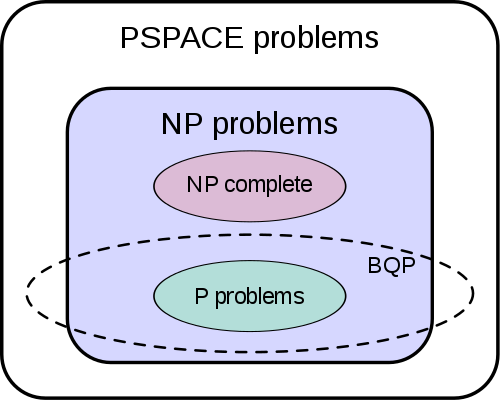
\includegraphics[width=\linewidth]{gfx/BQP_complexity_class_diagram}
     \caption{\footnotesize Wikipedia/BQP}
    \end{figure}
 \end{columns}
 
%  \begin{center}
%   \visible<5->{\alert{Number of quantum algorithms is very limited}}
%  \end{center}

\vspace{\floatsep}

\visible<5->{
\footnotesize{
\fullcite{brandao_quantum_2016}

\fullcite{van_apeldoorn_quantum_2017}
}
}
 
\end{frame}



\section{Arora-Kale algorithm}

\begin{frame}{Semidefinite Programs}
 \begin{columns}
  \column{0.5\linewidth}
  Primal problem:
  \begin{align*}
    \textbf{max} & \quad \Tr(CX) \\
    \textbf{s.t.} & \quad \Tr(A_j X) \leq b_j,\;\forall j \in [m] \\
		      & \quad X \geq 0.
  \end{align*}
  \column{0.5\linewidth}
  Dual problem:
  \begin{align*}
    \textbf{min} & \quad b^T y \\
    \textbf{s.t.} & \quad \sum_{j=1}^m y_j A_j - C \geq 0, \\
		      & \quad y \geq 0.
  \end{align*}
 \end{columns}
 
 \vspace{2\floatsep}
 
 $A_1,\dots,A_m,C$ are Hermitian $n\times n$ matrices and $b\in\R^m$.
 
 \vspace{2\floatsep}
 
 \structure{Assumptions:} $\|C\|, \|A_j\| \leq 1$ and $A_1 = I$, $b_1 = R$
\end{frame}


\begin{frame}{Matrix Multiplicative Weight Method}

\structure{Input:} Parameter $\eta \in (0,1]$, number of rounds $T\in\N$, dimension $d$

\begin{center}
\begin{tikzpicture}[>=stealth]
 \node [draw=structure.fg, thick, ellipse, align=center] (P) at (-2.5,0) {Player};
 \node [draw=structure.fg, thick, ellipse, align=center] (A) at (2.5,0) {Adversary};
 \draw [<-,thick] (P) to [bend right] (A) node[below=1cm, midway, align=center] {matrix $-I\leq M \leq I$ };
 \draw [<-,thick] (A) to [bend right] (P) node[above=1cm, midway] {density matrix $\rho$};
 
 \node at (4,-1.3) {\structure{Loss:} $\Tr(M\rho)$};
\end{tikzpicture}
\end{center}

\structure{Strategy:} Take $\rho^{(1)} = I/n$. For every $t$: 
\begin{enumerate}
 \item send $\rho^{(t)}$, obtain $M^{(t)}$
 \item update:
 \begin{equation*}
  \rho^{(t+1)} = \frac{\exp\left(-\eta \sum_{\tau=1}^t M^{(\tau)}\right) }{\Tr \exp\left(-\eta \sum_{\tau=1}^t M^{(\tau)}\right)}
 \end{equation*}

\end{enumerate}
 
\end{frame}

\begin{frame}{Matrix Multiplicative Weight Method}

\structure{Strategy:} Take $\rho^{(1)} = I/n$. For every $t\in[T]$: 
\begin{enumerate}
 \item send $\rho^{(t)}$, obtain $M^{(t)}$
 \item update: $\rho^{(t+1)} = \exp\left(-\eta \sum_{\tau=1}^t M^{(\tau)}\right)/\Tr(\dots)$
\end{enumerate}

\structure{$\Rightarrow$ Upper bound on total loss in the game \footcite{Arora2016}}

\begin{tikzpicture}[>=stealth,transform canvas={scale=0.6},shift={(15cm,-1cm)}]
 \node [draw=structure.fg, thick, ellipse, align=center] (P) at (-2.5,0) {Player};
 \node [draw=structure.fg, thick, ellipse, align=center] (A) at (2.5,0) {Adversary};
 \draw [<-,thick] (P) to [bend right] (A) node[below=1cm, midway, align=center] {matrix $-I\leq M \leq I$ };
 \draw [<-,thick] (A) to [bend right] (P) node[above=1cm, midway] {density matrix $\rho$};
 
%  \node at (4,-1.5) {\structure{Loss:} $\Tr(M^{(t)}\rho^{(t)})$};
\end{tikzpicture}

\vspace{\floatsep}

\begin{corollary}
 If $\Tr\left(M^{(t)}\rho^{(t)}\right)\geq 0$ $\forall t\in[T]$, then it holds
 \begin{equation*}
  \lambda_\mathrm{min}\underbrace{\left(\frac{1}{T} \sum_{t=1}^T M^{(t)} \right)}_{\text{almost psd!}} \geq -\eta - \frac{\ln(n)}{\eta T}
 \end{equation*}

\end{corollary}
 
\end{frame}

\begin{frame}{From MMW to a SPD Solver}

Given a guess $\alpha$ for the dual OPT value, we will construct a dual solution:

\vspace{\floatsep}

\structure{$\oracle(\rho)$} returns a vector $y\in\R^m_{\geq 0}$ such that
\begin{enumerate}
 \item $b^Ty \leq \alpha$
 \item$\Tr\left(\sum_{j=1}^m y_j A_j - C \right)\rho  \geq 0$
\end{enumerate}

\vspace{\floatsep}

The \structure{adversary's response} has to be normalised:
\begin{equation*}
 M = \frac{1}{w} \left( \sum_{j=1}^m y_j A_j - C \right)
\end{equation*}


\begin{tikzpicture}[transform canvas={scale=0.9},shift={(11cm,2.5cm)}]
 \node [draw=structure.fg, thick, ellipse, align=center] (A) at (0,0) {Adversary};
 \node [draw=alerted text.fg, inner sep=2mm, thick, align=center] (O) at (0,2) {$\oracle$};
 
 \draw [->,thick] (A) to [bend right] node[right] {$\rho$} (O);
 \draw [->,thick] (O) to [bend right] node[left] {$y$} (A);
\end{tikzpicture}

Here, $w$ is the \structure{width} of the ORACLE:
\begin{equation*}
 w = \sup \bigg\| \sum_{j=1}^m y_j A_j - C  \bigg\|
\end{equation*}


\end{frame}

\begin{frame}{From MMW to a SPD Solver}

\structure{Adversary:} Let $y^{(t)}=\oracle(\rho^{(t)})$ and respond 
\begin{equation*}
 M^{(t)}= \frac{1}{w} \left( \sum_{j=1}^m y^{(t)}_j A_j - C \right)
\end{equation*}

\begin{tikzpicture}[transform canvas={scale=0.9},shift={(11cm,1cm)}]
 \node [draw=structure.fg, thick, ellipse, align=center] (A) at (0,0) {Adversary};
 \node [draw=alerted text.fg, inner sep=2mm, thick, align=center] (O) at (0,2) {$\oracle$};
 
 \draw [->,thick] (A) to [bend right] node[right] {$\rho$} (O);
 \draw [->,thick] (O) to [bend right] node[left] {$y$} (A);
\end{tikzpicture}

\vspace{\floatsep}

By MMW, the average $\tilde{y}=\frac 1 T \sum_{t=1}^T y^{(t)} $ is \structure{almost dual feasible}:
\begin{equation*}
 - \left( \eta + \frac{\ln(n)}{\eta T}\right) I \leq \frac{1}{T} \sum_{t=1}^T M^{(t)} = \frac 1 w \left(\sum_{j=1}^m \tilde{y}_j A_j - C \right)
\end{equation*}

\vspace{\floatsep}

Since $A_1=I$, increasing $\tilde{y}_1$ turns this matrix psd.

\end{frame}

\begin{frame}{The Arora-Kale Meta-Algorithm}
 See blackboard \dots
\end{frame}

\begin{frame}{The $\oracle$}
 \structure{Recall:} $\oracle(\rho)$ returns a vector $y\in\R^m_{\geq 0}$ such that
 \begin{equation*}
  b^T y \leq \alpha \qquad\text{and}\qquad \Tr\left(\sum_{j=1}^m y_j A_j - C \right)\rho  \geq 0
 \end{equation*}
 
 \vspace{\floatsep}
 
 Runtime of Arora-Kale \structure{depends strongly} on the ORACLE via
 \begin{itemize}
  \item its concrete implementation
  \item its \structure{width} $w = \sup \| \sum_{j=1}^m y_j A_j - C  \|$ by the needed iterations
 \end{itemize}
 
 \vspace{\floatsep}

 Note: For a ORACLE with bounded output $\|y\|_1 \leq r$ we have $w \leq r + 1$.
 

\end{frame}

% ************************************
\section{Quantum Speed-Ups}
% ************************************


\begin{frame}{The Quantum Speed-Ups}
 \begin{block}{Calculating the input of the Oracle:}
  Estimate $\Tr(A\rho)$ for a hermitian matrix $A$ and a density operator $\rho$.
 \end{block}
 
 \begin{block}{A fast implementation of the Oracle:}
  Find a feasible solution of a linear programm.
 \end{block}
\end{frame}

\subsection{The input of the Oracle:}

\begin{frame}{First Speed-Up: Input of the Oracle}
 \begin{block}{Problem:}
  \textbf{Input:} Hermitian matrices $A,H$ \\
  \textbf{Output:} Approximation of $\Tr(A\rho)$ with $\rho=\frac{e^{-H}}{\Tr(e^{-H})}$
 \end{block}
 
 \begin{block}{Note:}
  The output is the \structure{probability} of a qubit being $0$.\\
  \alert{$\Rightarrow$ We need to construct a quantum circuit, which turns a specific register (e.g. $\ket{0\ldots 0}$) into one where the first qubit is as needed.}
 \end{block} 
\end{frame}

\begin{frame}{The input of the Oracle: Linear programming}
\begin{block}{LP as a special case of SDP}
All matrices are diagonal matrices.\\
\alert{Calculation of $\Tr(Ae^{-H})$ becomes much easier:}

\begin{equation*}
\Tr(Ae^{-H})=\sum_{i=1}^n A_{ii}e^{-H_{ii}}
\end{equation*}

\end{block}

\vspace{1cm}

\structure{Idea:} Calculate a binary approximation using \structure{arithmetic circuits} first, then \structure{transform} the first qubit accordingly.

\end{frame}

\begin{frame}{The input of the Oracle: Linear programming}
We start by applying Hadamard gates to \structure{$\ket{0\ldots 0}$} to get the state:
\begin{equation*}
\structure{\frac{1}{\sqrt{n}}\sum_{i=1}^n\ket{i}}
\end{equation*}
\pause
To this we apply the input oracles $O_H\ket{i}\ket{z}=\ket{i}\ket{z\oplus H_{ii}}$ to get
\begin{equation*}
\frac{1}{\sqrt{n}}\sum_{i=1}^n\ket{i}\structure{\ket{H_{ii}}\ket{A_{ii}}}
\end{equation*}
\pause
Now we can apply an \structure{arithmetic circuit} to calculate
\begin{equation*}
\frac{1}{\sqrt{n}}\sum_{i=1}^n\ket{i}\ket{H_{ii}}\ket{A_{ii}}\structure{\ket{\beta_i}}
\end{equation*}
with $\beta_i\approx\arcsin\left(\sqrt{A_{ii}e^{-H_{ii}}}\right)/\pi$.

\end{frame}

\begin{frame}{The input of the Oracle: Linear programming}
\begin{equation*}
\frac{1}{\sqrt{n}}\sum_{i=1}^n\ket{i}\ket{H_{ii}}\ket{A_{ii}}\ket{\beta_i} \text{, with } \beta_i\approx\arcsin\left(\sqrt{A_{ii}e^{-H_{ii}}}\right)/\pi
\end{equation*}

\vspace{1cm}

Now we can apply the \structure{transformation}
\begin{equation*}
\ket{1}\ket{\beta}\to (\sin(\pi\beta)\ket{0}+\cos(\pi\beta)\ket{1})\ket{\beta}
\end{equation*}
to an ancilla qubit:

\begin{equation*}
\frac{1}{\sqrt{n}}\sum_{i=1}^n\structure{\left(\sqrt{A_{ii}e^{-H_{ii}}}\ket{0}+\sqrt{1-A_{ii}e^{-H_{ii}}}\ket{1}\right)}\ket{i}\ket{H_{ii}}\ket{A_{ii}}\ket{\beta_i}
\end{equation*}
\end{frame}

\begin{frame}
\begin{equation*}
\frac{1}{\sqrt{n}}\sum_{i=1}^n\left(\sqrt{A_{ii}e^{-H_{ii}}}\ket{0}+\sqrt{1-A_{ii}e^{-H_{ii}}}\ket{1}\right)\ket{i}\ket{H_{ii}}\ket{A_{ii}}\ket{\beta_i}
\end{equation*}

The \structure{probability} that this state's first qubit is 0 is:
\begin{equation*}
\left\|\frac{1}{\sqrt{n}}\sum_{i=1}^n\sqrt{A_{ii}e^{-H_{ii}}}\ket{i}\right\|^2=\frac{1}{n}\sum_{i=1}^n A_{ii}e^{-H_{ii}}=\frac{1}{n}\Tr(Ae^{-H})
\end{equation*}
\end{frame}

\begin{frame}{The input of the Oracle: SDP}

\structure{Idea: } Construct circuits for $\sqrt{A}$ and $\sqrt{e^{-H}}=e^{-H/2}$, then evaluate $\sum_i \bra{i}\sqrt{A}\sqrt{e^{-H}}\ket{i}$ to get the trace.

\begin{block}{Problem: These matrices are not unitary}
Instead we construct for the norm-decreasing maps $B=\sqrt{A}$ and $e^{-H/2}$ circuits with
\begin{equation*}
U_B\ket{0}\ket{i}=\ket{0}B\ket{i}+\ket{1}*
\end{equation*}
\pause
We can apply both operations to the same $\ket{i}$ by using different ancilla qubits for each operation:
\begin{align*}
U_{\sqrt{A}}&U_{e^{-H/2}}\ket{0}\ket{0}\ket{i}\\
&=U_{\sqrt{A}}(\ket{0}\ket{0}e^{-H/2}\ket{i}+\ket{0}\ket{1}*)\\
&=\ket{0}\ket{0}\sqrt{A}e^{-H/2}\ket{i}+\ket{0}\ket{1}*+\ket{1}\ket{0}*+\ket{1}\ket{1}*
\end{align*}
\end{block}

\end{frame}

\begin{frame}{The input of the Oracle: SDP}
When we now apply this circuit to $\ket{0}\ket{0}\sum_{i=1}^n \frac{\ket{i}\ket{i}}{\sqrt{n}}$, then is the probability that the first two qubits are zero
\begin{align*}
\left\|\sum_{i=1}^n\frac{\left(\sqrt{A}e^{-H/2}\ket{i}\right)\ket{i}}{\sqrt{n}} \right\|^2 & \\ 
=&\frac 1 n \sum_{i,j=1}^n \left( \bra{j}\bra{j}\left(e^{-H/2}\right)^\dagger\sqrt{A}^\dagger\right)\sqrt{A}e^{-H/2}\ket{i}\ket{i} \\
=&\frac{1}{n}\sum_{i=1}^n \bra{i}\left(e^{-H/2}\right)^\dagger\sqrt{A}^\dagger\sqrt{A}e^{-H/2}\ket{i}\\
=&\frac{1}{n}\Tr\left(\sqrt{A}\sqrt{A}e^{-H/2}e^{-H/2}\right)\\
=&\frac{1}{n}\Tr\left(Ae^{-H}\right)
\end{align*}
\end{frame}

\begin{frame}{Constructing circuits for  $\sqrt{A}$ and $e^{-H/2}$}
\begin{block}{How do we construct these circuits?}

$\sqrt{H}$ and $e^{H}$ are functions of hamiltonians:

\begin{equation*}
f(H)=f(U \, \mathrm{Diag} (\lambda_1,\ldots, \lambda_n) U^\dagger)=U \, \mathrm{Diag}(\tilde{f}(\lambda_1),\ldots,\tilde{f}(\lambda_n))U^\dagger
\end{equation*}

\begin{itemize}
 \item[$\to$] Polynomial approximation of $\tilde{f}$\\
 \item[$\to$] Fourier series \\
 \item[$\to$] Quantum circuit \\
 \item[$\to$] Extension to apply to hermitian matrices
\end{itemize}
\end{block}
\end{frame}

\subsection{The Oracle}

%TODO Layout
\begin{frame}{The Oracle: Problem definition}
\structure{Input: } $\alpha\in\R$, $r\in \R_{\geq 0}$, $a\in \R^m$ with $a_j\approx \Tr(A_j \rho)$, $b\in \R^m$, $c\approx \Tr(C\rho)-\varepsilon$\\
\vspace{1cm}
\structure{Output: } $y\in \mathbb{R}^m$ with:
%TODO Fix spacing
% \begin{columns}
% \column{0.5\linewidth}
\begin{align*}
\|y\|_1&\leq r & \omit\rlap{\structure{Compared to the dual SDP}}\\
b^T y&\leq \alpha&\min \quad &b^T y\\
a^T y&\geq c& \text{s.t. } &\sum_{j=1}^m y_j A_j - C\succeq 0\\
y&\geq 0 & &y\geq 0
\end{align*}
% \column{0.5\linewidth}
% \begin{block}{Compared to the dual SDP:}
% \begin{align*}
% \min\quad&b^T y\\
% \text{s.t. }&\sum_{j=1}^m y_j A_j - C\succeq 0\\
% &y\geq 0
% \end{align*}
% \end{block}

% \end{columns}
\end{frame}

\begin{frame}{Simplifying the problem}
Substituting \structure{$y=Nq$} with $N=\|y\|_1$ and $\|q\|_1=1$ results in:

%Some ugly magic for rcases inside of align
\begin{equation*}
 \begin{split}
  b^T q&\leq \alpha/N\\
  a^T q&\geq c/N\\
  \begin{aligned}
   \|q\|_1\\
   q
  \end{aligned}
  &
  \begin{rcases*}
   =1\\
   \geq 0
  \end{rcases*} \text{\structure{convex combination} coefficients}  \\
  0&<N\leq r
 \end{split}
\end{equation*}
\end{frame}

\begin{frame}{Simplifying the problem}
\begin{block}{Problem: two-dimensional interpretation}
Find the \structure{convex combination} of a point $P\in\mathrm{conv}\{p_i=(b_i,a_i)\}$, which lies to the \structure{upper left} of $(\alpha/N, c/N)$ for an $0<N\leq r$.
\end{block}

\vspace{1cm}

Define $G_N$ as the upper-left quadrant starting at $(\alpha/N, c/N)$.
Define $G$ as the union of all $G_N$ with $0<N\leq r$.

\end{frame}

\begin{frame}{Understanding the area $G$}


\begin{columns}
\column{0.36\linewidth}

\raggedleft
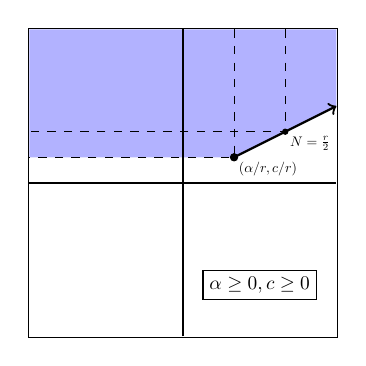
\begin{tikzpicture}[scale=0.65]%[shift={(11cm,-1.5cm)}]
\contourlength{0.5mm};

\coordinate[label={[scale=0.5]below right: {$(\alpha/r,c/r)$}}] (ac) at (1,1/2);
\coordinate[label={[scale=0.5]below right: {$N=\frac{r}{2}$}}]  (ac2) at (2,1);
\coordinate													    (ac3) at (3,3/2);

\fill[blue!30!white] (ac)--(ac -| -3,0)--(-3,3)--(ac3 |- 0,3)--(ac3)--cycle;

\draw[thick] (-3,0)--(3,0);
\draw[thick] (0, -3)--(0,3);
\draw[dashed] (ac |- 0,3) -- (ac) -- (ac -| -3,0);
\draw[dashed] (ac2 |- 0,3) -- (ac2) -- (ac2 -| -3,0);

\filldraw (ac) circle(0.07);
\filldraw (ac2) circle(0.05);

\draw[->, thick] (ac)--(ac3);

\node[scale=0.7,draw] at (1.5,-2) {$\alpha\geq 0, c\geq 0$};
\draw (current bounding box.north east) rectangle (current bounding box.south west);
\end{tikzpicture}


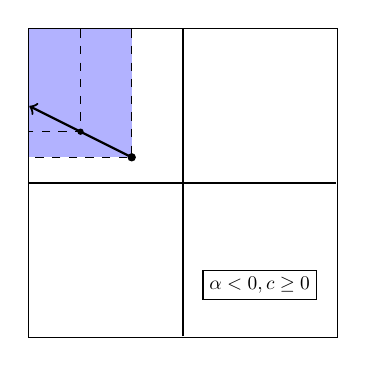
\begin{tikzpicture}[scale=0.65]%[shift={(11cm,-1.5cm)}]
\contourlength{0.5mm};

\coordinate (ac) at (-1,1/2);
\coordinate (ac2) at (-2,1);
\coordinate	(ac3) at (-3,3/2);

\fill[blue!30!white] (ac)--(ac -| -3,0)--(-3,3)--(ac |- 0,3)--cycle;

\draw[thick] (-3,0)--(3,0);
\draw[thick] (0, -3)--(0,3);
\draw[dashed] (ac |- 0,3) -- (ac) -- (ac -| -3,0);
\draw[dashed] (ac2 |- 0,3) -- (ac2) -- (ac2 -| -3,0);

\filldraw (ac) circle(0.07);
\filldraw (ac2) circle(0.05);

\draw[->, thick] (ac)--(ac3);

\node[scale=0.7,draw] at (1.5,-2) {$\alpha < 0, c\geq 0$};
\draw (current bounding box.north east) rectangle (current bounding box.south west);
\end{tikzpicture}
\column{0.36\linewidth}

\raggedright
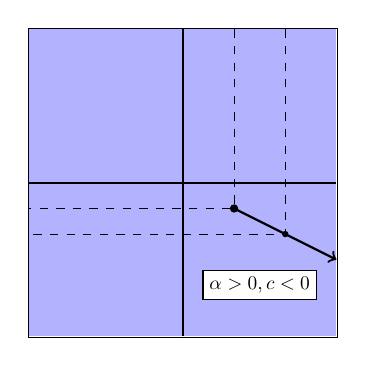
\begin{tikzpicture}[scale=0.65]%[shift={(11cm,-1.5cm)}]
\contourlength{0.5mm};

\coordinate (ac) at (1,-1/2);
\coordinate (ac2) at (2,-1);
\coordinate	(ac3) at (3,-3/2);

\fill[blue!30!white] (-3,-3)--(-3,3)--(3,3)--(3,-3)--cycle;

\draw[thick] (-3,0)--(3,0);
\draw[thick] (0, -3)--(0,3);
\draw[dashed] (ac |- 0,3) -- (ac) -- (ac -| -3,0);
\draw[dashed] (ac2 |- 0,3) -- (ac2) -- (ac2 -| -3,0);

\filldraw (ac) circle(0.07);
\filldraw (ac2) circle(0.05);

\draw[->, thick] (ac)--(ac3);

\node[scale=0.7,draw, fill=white] at (1.5,-2) {$\alpha > 0, c < 0$};
\draw (current bounding box.north east) rectangle (current bounding box.south west);
\end{tikzpicture}


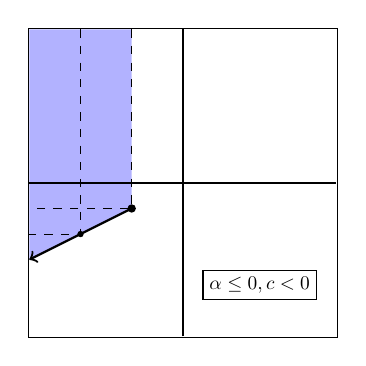
\begin{tikzpicture}[scale=0.65]%[shift={(11cm,-1.5cm)}]
\contourlength{0.5mm};

\coordinate (ac) at (-1,-1/2);
\coordinate (ac2) at (-2,-1);
\coordinate	(ac3) at (-3,-3/2);

\fill[blue!30!white] (ac)--(ac |- -3,3)--(-3,3)--(ac3)--cycle;

\draw[thick] (-3,0)--(3,0);
\draw[thick] (0, -3)--(0,3);
\draw[dashed] (ac |- 0,3) -- (ac) -- (ac -| -3,0);
\draw[dashed] (ac2 |- 0,3) -- (ac2) -- (ac2 -| -3,0);

\filldraw (ac) circle(0.07);
\filldraw (ac2) circle(0.05);

\draw[->, thick] (ac)--(ac3);

\node[scale=0.7,draw] at (1.5,-2) {$\alpha \leq 0, c < 0$};
\draw (current bounding box.north east) rectangle (current bounding box.south west);
\end{tikzpicture}

\column{.28\textwidth}
If $\alpha > 0, c < 0$, then is $G=\R^2$. 

\vspace{1cm}
Otherwise $G$ is the intersection of two half-planes.

\end{columns}

\end{frame}

\begin{frame}{2-sparse solutions}
\begin{tikzpicture}
\contourlength{0.5mm};
\shade[lower right=blue!60!white] (0,0) rectangle (3,3);
\node at (1,2) {\contour{white}{$G_N$}};
\filldraw[thick, fill=red!20!white, fill opacity=0.3] (0,-1)--(4,3)--(6,2)--(4,-2)--(2,-2)--cycle;
\draw[red, thick] (1,0)--(3,2);
\node[anchor=south] at (4,3) {$Q=\mathrm{conv}\{p_i|1\leq i \leq m\}$};
\draw (0,-1)--(6,2)--(2,-2)--(4,3)--(4,-2)--cycle;
\filldraw (2.5,0.5) circle(0.07) node[anchor=south east]{\contour{white}{$P$}};
\filldraw (3,0) circle(0.07) node[anchor=north west]{\contour{white}{$(\alpha/N,c/N)$}};
\node[text width=5cm] at (9,0) 
	{If there is no $p_i\in G_N$,\\
	but there is a $P\in G_N\cap Q$,\\
	then $\partial Q\cap G_N\neq \emptyset$.\\ 
	\vspace{0.5cm}
	In particular, there is a line with $\overline{p_i p_j}\cap G_N\neq\emptyset$.\\
	\vspace{0.5cm}
	That means we can always find a 2-sparse solution $q$.};
\end{tikzpicture}
\end{frame}



\begin{frame}{The algorithm}
\begin{algorithmic}
\If{$\alpha\geq 0$ and $c\leq 0$}
	\Comment{Check if \structure{$G=\R^2$}}
    \State \Return $y=0$
    \pause
\ElsIf{$\exists i: p_i\in G$}
	\Comment{Check if a \structure{corner} is in $G$}
    \State \Return $y=Ne_i$ with $N=c/a_i$
    \pause
\Else
	\Comment{Search a \structure{2-sparse} solution}
	\State Find $j,k$ such that $\overline{p_j p_k}\cap G\neq \emptyset$
	\If{Such $j,k$ exist}
		\State Calculate a fitting convex combination $q$ and scalar $N$
		\State \Return $y=Nq$
	\Else
		\State \Return	No $y$ found.
	\EndIf
\EndIf
\end{algorithmic}
\end{frame}

\begin{frame}{How to find $j,k$ with $\overline{p_j p_k}\cap G\neq \emptyset$}
\begin{tikzpicture}
\contourlength{0.5mm};
\coordinate[label=below left:$L_1$] (L1) at (0,0);
\coordinate[label=above right:$L_2$] (L2) at (3,3);
\coordinate[label=below right:{$(\alpha/r,c/r)$}] (g) at (3,0);
\coordinate[label=below left:$p_j$] (pj) at (1,-1);
\coordinate[label=above right:$p_k$] (pk) at (4,2);

\shade[lower right=blue!60!white] (L1) rectangle (3,3);
\draw[thick] (g)--(L1);
\draw[thick] (g)--(L2);
\node at (1,2) {\contour{white}{$G$}};
\filldraw (g) circle(0.05);
\filldraw (pj) circle(0.05);
\filldraw (pk) circle(0.05);
\draw (g)--(pj);
\draw (g)--(pk);
\draw[dashed] (pj)--(pk);

\begin{scope}
\path[clip] (g) -- (pj) -- (L1);
\draw (g) circle (0.8);
\end{scope}
%\node[scale=0.5] at (2.3,-0.1)  {$\sphericalangle p_j L_1$};

\begin{scope}
\path[clip] (g) -- (L1) -- (L2);
\draw (g) circle (0.6);
\end{scope}
%\node[scale=0.5] at (2.6,0.2) {$\sphericalangle L_1 L_2$};

\begin{scope}
\path[clip] (g) -- (L2) -- (pk);
\draw (g) circle (0.8);
\end{scope}
%\node[scale=0.5] at (3.2,0.9) {$\sphericalangle L_2 p_k$};

\node[text width=5.5cm] at (8,1) 
	{The angle $\sphericalangle L_1 L_2$ is constant.\\
	\vspace{0.5cm}
	The line $\overline{p_j p_k}$ crosses $G$ if and only if:\\
	$\sphericalangle p_j L_1+\sphericalangle L_1 L_2
	    +\sphericalangle L_2 p_k\leq \pi$\\
	\vspace{0.5cm}
	\alert{$\Rightarrow$ Minimize $\sphericalangle p_j L_1$ and 
		$\sphericalangle L_2 p_k$   seperately!}};
\end{tikzpicture}
\end{frame}

\begin{frame}{Where is the quantum speed-up?}
\begin{block}{Step 2: Check if there is a $p_i\in G$}
If we implement the function $i\to$"Is $p_i\in G$?" as a quantum circuit, then \structure{Grover search} can be used to find such a $p_i$ in $\mathcal{O}(\sqrt{m})$.
\end{block}

\begin{block}{Step 3: Minimize the angles $\sphericalangle p_j L_1$ and 
		$\sphericalangle L_2 p_k$}
If we implement the functions $i\to\sphericalangle p_i L_1$ and $i\to \sphericalangle L_2 p_k$ as quantum circuits, then the \structure{quantum minimum-finding} algorithm of \structure{Dürr and Høyer} can be used to minimize them in $\mathcal{O}(\sqrt{m})$.
\end{block}
\end{frame}

%Chapter 4?
\subsection{Runtime of the SDP solver}
\begin{frame}{Runtime of the algorithm}
\begin{itemize}
\item calculating \structure{$\Tr(A_j\rho)$} during iteration $t$:
\begin{equation*}
\tilde{\mathcal{O}}\left(\sqrt{n}s^2\frac{\eta t^3 Rr}{\varepsilon}\right)
\end{equation*}
\pause
\item \structure{one iteration}: $\tilde{\mathcal{O}}(\sqrt{m})$ uses of $\Tr(A_j\rho)$ in the Oracle:
\begin{equation*}
\tilde{\mathcal{O}}\left(\sqrt{nm}s^2\frac{\eta t^3 Rr}{\varepsilon}\right)
\end{equation*}
\end{itemize}
\end{frame}

\begin{frame}{Runtime of the algorithm}
Number of iterations $T=\tilde{\mathcal{O}}\left(\frac{R^2 r^2}{\varepsilon^2}\right)$, $\eta=\sqrt{\frac{\ln(n)}{T}}$

\vspace{1cm} 

\structure{Total runtime for SDP}:

\begin{align*}
\tilde{\mathcal{O}}\left(\sum_{t=1}^T \sqrt{nm}s^2\frac{\eta t^3 Rr}{\varepsilon}\right)&=\tilde{\mathcal{O}}\left(\sqrt{nm}s^2\frac{\eta T^4 Rr}{\varepsilon}\right)\\
&=\tilde{\mathcal{O}}\left(\sqrt{nm}s^2\left(\frac{Rr}{\varepsilon}\right)^8\right)
\end{align*}

\end{frame}

\begin{frame}{Runtime of the algorithm: LP}
Diagonal matrices have sparsity $s=1$, and we can use the LP case for calculating $\Tr(A_j\rho)$.

\vspace{1cm} 

\structure{Total runtime for LP}:

\begin{align*}
\tilde{\mathcal{O}}\left(\sqrt{nm}\left(\frac{Rr}{\varepsilon}\right)^5\right)
\end{align*}

\end{frame}

\begin{frame}{Comparing quantum with classical runtimes}
Best known \structure{classical general SDP-solver}:
\begin{equation*}
\tilde{\mathcal{O}}(m(m^2+n^\omega+mns)) \text{ with } \omega\in[2,2.373)
\end{equation*}

\vspace{\floatsep}

This \structure{quantum SDP solver}:
\begin{equation*}
\tilde{\mathcal{O}}\left(\sqrt{nm}s^2\left(\frac{Rr}{\varepsilon}\right)^8\right)
\end{equation*}

\vspace{\floatsep}

\structure{Arora-Kale with \emph{classical} ORACLE}:
\begin{equation*}
 \tilde{\mathcal{O}}\left(nms \left(\frac{Rr}{\varepsilon}\right)^4 + ns \left(\frac{Rr}{\varepsilon}\right)^7 \right).
\end{equation*}

\end{frame}
% ************************************
\section{Limitations}
% ************************************

\begin{frame}{Limitations}

 \structure{Runtime}
 \begin{itemize}
  \item Speed-up in $nm$ but worse scaling in  $Rr/\varepsilon$
  \item No known SDP examples with $nm \gg  Rr/\varepsilon$ \dots
 \end{itemize}
 
  \vspace{2\floatsep}
  
  \pause
 
  \structure{General oracles are slow}
 \begin{itemize}
  \item Sparse oracles have necessarily a large width for solution with at least $l$ non-zeros \\ $\Rightarrow$ For the previous oracle: runtime $\Omega( l^4 \sqrt{nm} s^2)$
  \item General width bounds can lead to bad runtimes 
 \end{itemize}
 \structure{$\Rightarrow$ Adapt to specific SDPs using quantum oracles}


\end{frame}

\begin{frame}{Conclusions}

\structure{Results}
\begin{itemize}
 \item Quantum algorithm with a completely new application
 \item Quadratic speed-up in dimensions
 \item \dots but worse scaling in other parameters
\end{itemize}

\vspace{\floatsep}

\pause

\structure{Outlook}
\begin{itemize}
 \item Further evolution on quantum SDP algorithms with better bounds
 \item Development of new quantum algorithms
\end{itemize}



\end{frame}


\appendix
% bibliography
\nocite{*}
\frame[allowframebreaks]{\printbibliography}

%Binary->amplitude
\begin{frame}{Transforming a binary value into a qubit amplitude}
Let $b\in [0,1]$ be the value we want as the \structure{probability} of a qubit being 0
\begin{itemize}
\item calculate a \structure{binary approximation} $b_0.b_1b_2b_3\ldots b_t$ of $\beta=\arcsin(\sqrt{b})/\pi$
\item start with the register $\ket{1}\ket{\beta}=\ket{1}\ket{b_0}\ket{b_1}\ldots\ket{b_t}$
\item apply $t$ \structure{controlled rotations} to the first qubit, rotating by $\pi 2^{-j}$ towards $\ket{0}$ if $b_j=1$
\end{itemize}
Afterwards our register is: 
\begin{align*}
&\left(\sin\left(\sum_{b_i=1} \pi 2^{-i}\right)\ket{0}
+\cos\left(\sum_{b_i=1} \pi 2^{-i}\right)\ket{1}\right)
 \ket{\beta}\\
=&\left(\sin\left(\pi\beta\right)\ket{0}
+\cos\left(\pi\beta\right)\ket{1}\right)
 \ket{\beta}\\
=&(\structure{\sqrt{b}}\ket{0}+\sqrt{1-b}\ket{1})\ket{\beta}
\end{align*}
For which the probability, that the first qubit is 0, is exactly $\|\sqrt{b}\ket{0}\|^2=b$.
\end{frame}

\end{document}
